	
\subsubsection{20.10.14}

\begin{enumerate}
	\item Time of beginning and ending of congregation:
	20:30 - 21:30
	\item Purposes of congregation:
	\begin{enumerate}
	  \item Correct the problem of servo.
	  
	  \item To fix transverse beams at the lift.
	  
    \end{enumerate}
    
	\item Work, that has been done:
	\begin{enumerate}
	  \item For correction of problem with servo we tried to make that before stop it slightly rotate to back. But it wouldn't work.
	  
      \item Г-shaped profile was cut on corners of needed length.
      
      \item Transverse beams were made. One from their was installed at robot.
      
      \begin{figure}[H]
      	\begin{minipage}[h]{0.47\linewidth}
        	\center{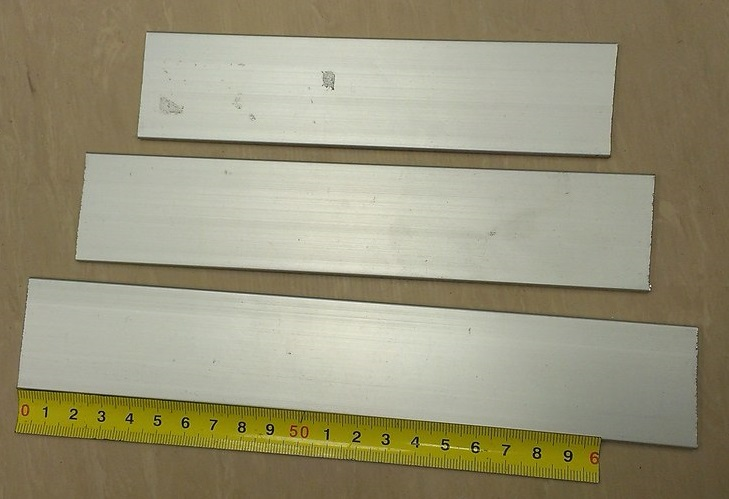
\includegraphics[scale=0.3]{days/20.10.14/images/01}}
      		\caption{Transverse beams}  
      	\end{minipage}
      	\hfill
      	\begin{minipage}[h]{0.47\linewidth}
      		\center{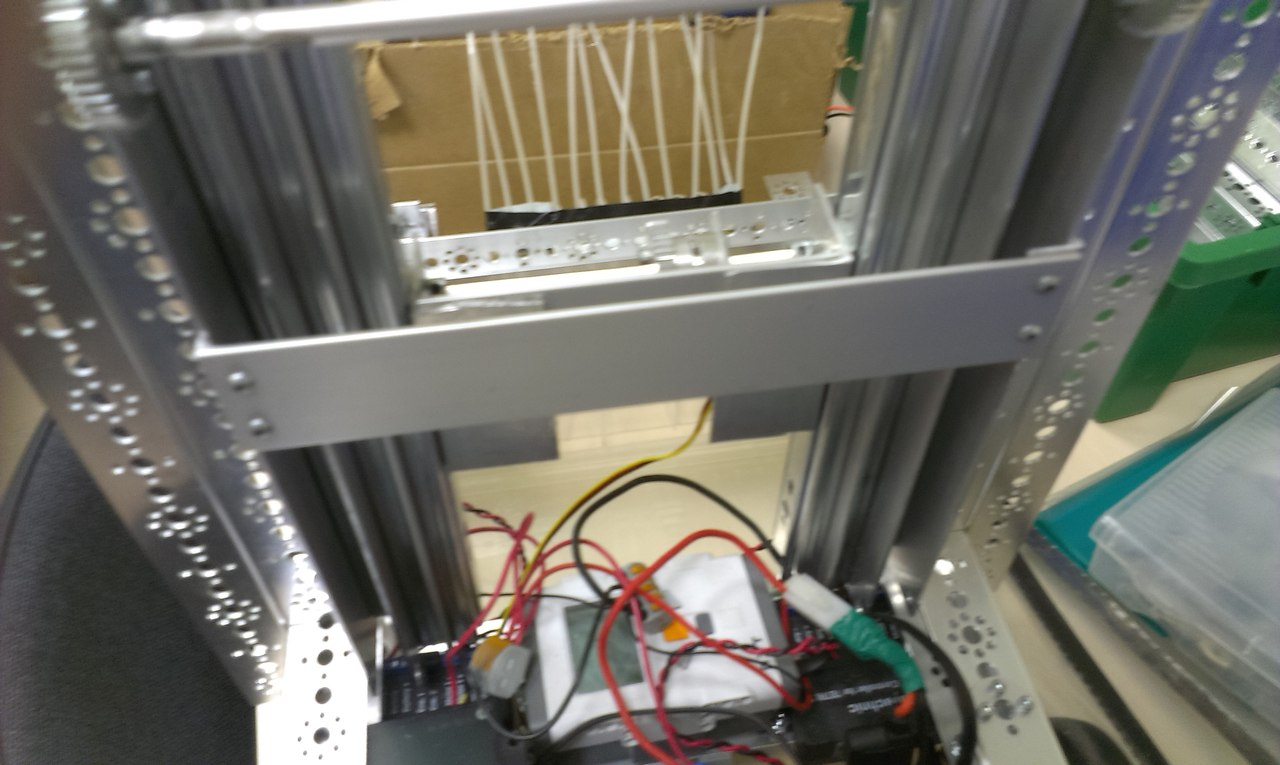
\includegraphics[scale=0.2]{days/20.10.14/images/02}}
      		\caption{Transverse beam that was installed at robot}
      	\end{minipage}
      \end{figure}
      
      \item Today we learned that 21 - 23 of November will the competition FTC in Sochi. It was decided that our team will take part in this competition.Until the next congregation every participants of team  will have to give an answer, will he be able to go to Sochi.
      
    \end{enumerate}
    
	\item Results: 
	\begin{enumerate}
	  \item Problem with servo not corrected.
	  
      \item All ready for fixing of transverse beams to guides.
      
      \item One transverse beam was installed.
      
    \end{enumerate}
    
	\item Tasks for the next congregations:
	\begin{enumerate}
	  \item Finish fastening transverse beams to guides of lift.
	  
	  \item Correct the problem with servo.
	  
	  \item Decide who can go to Sochi.
	 
    \end{enumerate}     
\end{enumerate}
\fillpage
